\lab{Bayesian Search}{Bayesian Search}
\objective{Understand how Bayesian methods can be used for search and rescue operations.}

In the past half century, statistical methods have seen a rise in popularity for search and rescue problems. \emph{Bayesian search theory} has been successfully used to find lost sea vessels and aircraft, including the USS \emph{Scorpion}, the MV \emph{Derbyshire}, the SS \emph{Central America}, and Air France Flight (AF) $447$. It was also used to search for a lost nuclear bomb after a B-52 bomber crashed in Spain in $1966$.

In this lab, we will simulate search procedures for the AF$447$ disaster, using our knowledge of Bayes' Theorem and estimations of ocean depth in the vicinity of the last point of radio contact with the flights captains.

On June $1^{\text{st}}$, $2009$, AF$447$ departed Rio de Janeiro, Brazil, flying to Paris, France. Air traffic controllers lost contact with the aircraft at $2$:$10$ AM, nearly halfway between South America and Western Africa. The location of final contact was approximately $2.98^{\circ} N, 30.59^{\circ} W$. Figure \ref{trajectory} shows the flight path (and part of the planned flight path) of AF$447$.

\begin{figure}[h]
\centering
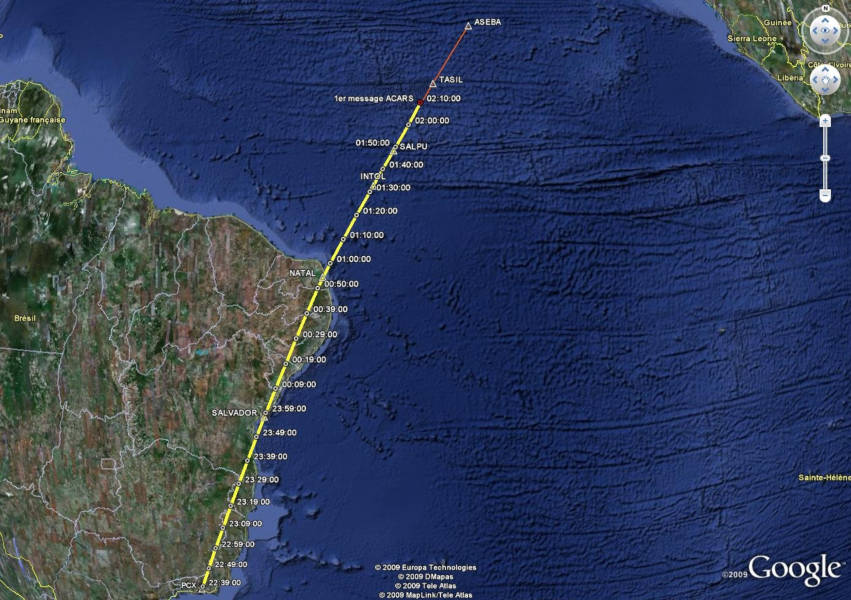
\includegraphics[width=\textwidth]{trajectory.jpg}
\caption{Flight path of AF$447$.}
\label{fig:trajectory}
\end{figure}

The search operations proved unsuccessful for nearly two years. After an unsuccessful first year of searching, the consulting company Metron was asked to develop a probabilistic search procedure to find the flight. Using Bayesian search methods, a large portion of AF$447$'s debris field was discovered within a week of resuming the search. Within a month, the black boxes were recovered.

Bayesian search theory consists of combining our belief of where a lost vessel should be located with our belief of our success of finding it in a location, should we search there. A simple way of expressing our belief of where a lost vessel should be found is with a probability distribution, centered at the last point of contact. Our belief of successfully finding the vessel in a given location can be a function of ocean depth (or, for a land based search, a function of density of foliage, difficulty of searching a mountainous region, etc.). We simplify this by discretizing the possible locations into a square grid.

Formally, let $A_{i}$ be the event that we successfully find the vessel when we search in location $i$, and let $B_{i}$ be the event that the vessel is in location $i$. Then let $p$ be a probability distribution for the location of the vessel over the grid, so $$p_{i} = \mathbb{P}(B_{i}).$$ Let $q$ be a set of $N$ Bernoulli parameters, each denoting the probability of success if we search in its location, i.e.
$$q_{i} = \mathbb{P}(A_{i} | B_{i}).$$ We also assume no chance of success in finding the vessel in location $i$ if it is \emph{not} located there.

This allows us to compute 
\begin{align*}
r_{i} & = \mathbb{P}(A_{i}) \\
& = \sum_{j} \mathbb{P}(A_{i} \cap B_{j}) \\
& = \sum_{j} \mathbb{P}(A_{i} | B_{j})\mathbb{P}(B_{j}) \\
& = \mathbb{P}(A_{i} | B_{i})\mathbb{P}(B_{i}) \\
& = p_{i}q_{i} \\
\end{align*}

We proceed by searching in location $k$, where $k = \text{argmax}_{i} r_{i}$.

\begin{problem}
Write a function that accepts two $20 \times 20$ arrays, $p$ and $q$, and returns the index pair $i,j$ of the next search location.
\end{problem}

If a search successful, then our search is over. If unsuccessful, we update our probabilities $p_{i}$ given our recent data $\theta$ (our unsuccessful attempt) according to Bayes Rule, which in this case, is
\begin{equation*}
\mathbb{P}(B_{i} \; | \; \theta) = \frac{\mathbb{P}(\theta \; | \; B_{i})\mathbb{P}(B_{i})}{\mathbb{P}(\theta \; | \; B_{i})\mathbb{P}(B_{i}) + \mathbb{P}(\theta \; | \; B_{i}^{c})\mathbb{P}(B_{i}^{c})}
\end{equation*}

This has two different solutions, depending on where we searched, yielding the following for our posterior probability:
\begin{equation*}
\tilde{p}_{i} = \begin{cases} \frac{(1-q_{i})p_{i}}{(1-q_{i})p_{i} + (1-p_{i})} = p_{i}\frac{1-q_{i}}{1-p_{i}q_{i}} & \mbox{if we searched in location } i \\ \frac{p_{i}}{(1-q_{i})p_{i} + (1-p_{i})} = \frac{p_{i}}{1-p_{i}q_{i}} & \mbox{if we searched in location } j \neq i \end{cases}
\end{equation*}

\begin{problem}
Write a function that accepts two $20 \times 20$ arrays, $p$ and $q$, as well as an index pair $i,j$ of search coordinates for the most recent unsuccessful search, and returns the posterior probabilities $\tilde{p}_{k,l}$ for each possible location $k,l$, where $1 \leq k,l \leq 20$.
\end{problem}

Using our computed posterior probability and our success probabilities, we compute $r$ again, and choose a search location, continuing this procedure until success.

\begin{problem}
Write a function to simulate the search procedure. It should accept two $20 \times 20$ arrays, $p$ and $q$, where $p$ is our initial prior on the location of the vessel and $q$ contains the probability of success for each grid location. It should also accept the actual location $i,j$ of the vessel. During the simulation process, assume that $q$ is correct, i.e. given that we search in location $i,j$, we will successfully find the vessel with probability $q_{i,j}$. The function should return the number of search iterations until success, as well as the location of the vessel (but don't hard code this!).
\end{problem}

We have roughly examined the ocean depths in the vicinity of the crash, and compute probabilities of successfully finding it in a location, given that we search there (this is simply a function of depth). We have also computed an initial prior on the location, with locations nearer the final point of contact having higher probabilities than locations further away. These are represented as $20 \times 20$ arrays, and are located in the files \texttt{depthProbs} and \texttt{prior}, respectively.

\begin{problem}
Unpickle the two files mentioned above, and test your previous function. Once it's working properly, write a function that runs the previous function $n\_sim$ times, and prints out the shortest search length, longest search length, and average search length. Test it with $n\_sim = 500$ at locations $9, 10$ and $12, 5$.
\end{problem}